\section{Person Discovery challenge}
\label{sec:challenge}


The goal of this challenge is to address the challenge of indexing people in the archive under real-world conditions,  (\emph{i.e.} using algorithms not relying on pre-existing labels or biometric models).

\mypartitle{Task overview.} Participants are provided with a collection of TV broadcast recordings pre-segmented into shots.
Each shot $s \in \shots$ has to be automatically tagged with the names of people both speaking and appearing at the same time during the shot: this tagging algorithm is denoted by $\hypLabels : \shots \mapsto \mathcal{P}(\hypNames)$.

The list of persons is not provided \emph{a priori}, and person biometric models (neither voice nor face) can not be trained on external. The only way to identify a person is by finding their name $n \in \hypNames$ in the audio (\emph{e.g.} using ASR) or visual (\emph{e.g.} using OCR) streams and associating them to the correct person (Fig. \ref{fig:evidence}). %This makes the task completely unsupervised (\emph{i.e.} using algorithms not relying on pre-existing labels or biometric models). 
%Because person names are detected and transcribed automatically, they may contain transcription errors to a certain extent (more on that later in Section~\ref{sec:metric}). 
We denote by $\refNames$ the set of all possible person names in the universe, correctly formatted as \texttt{firstname\_lastname} -- while $\hypNames$ is the set of hypothesized names.

\begin{figure}[tb]
 \centering
 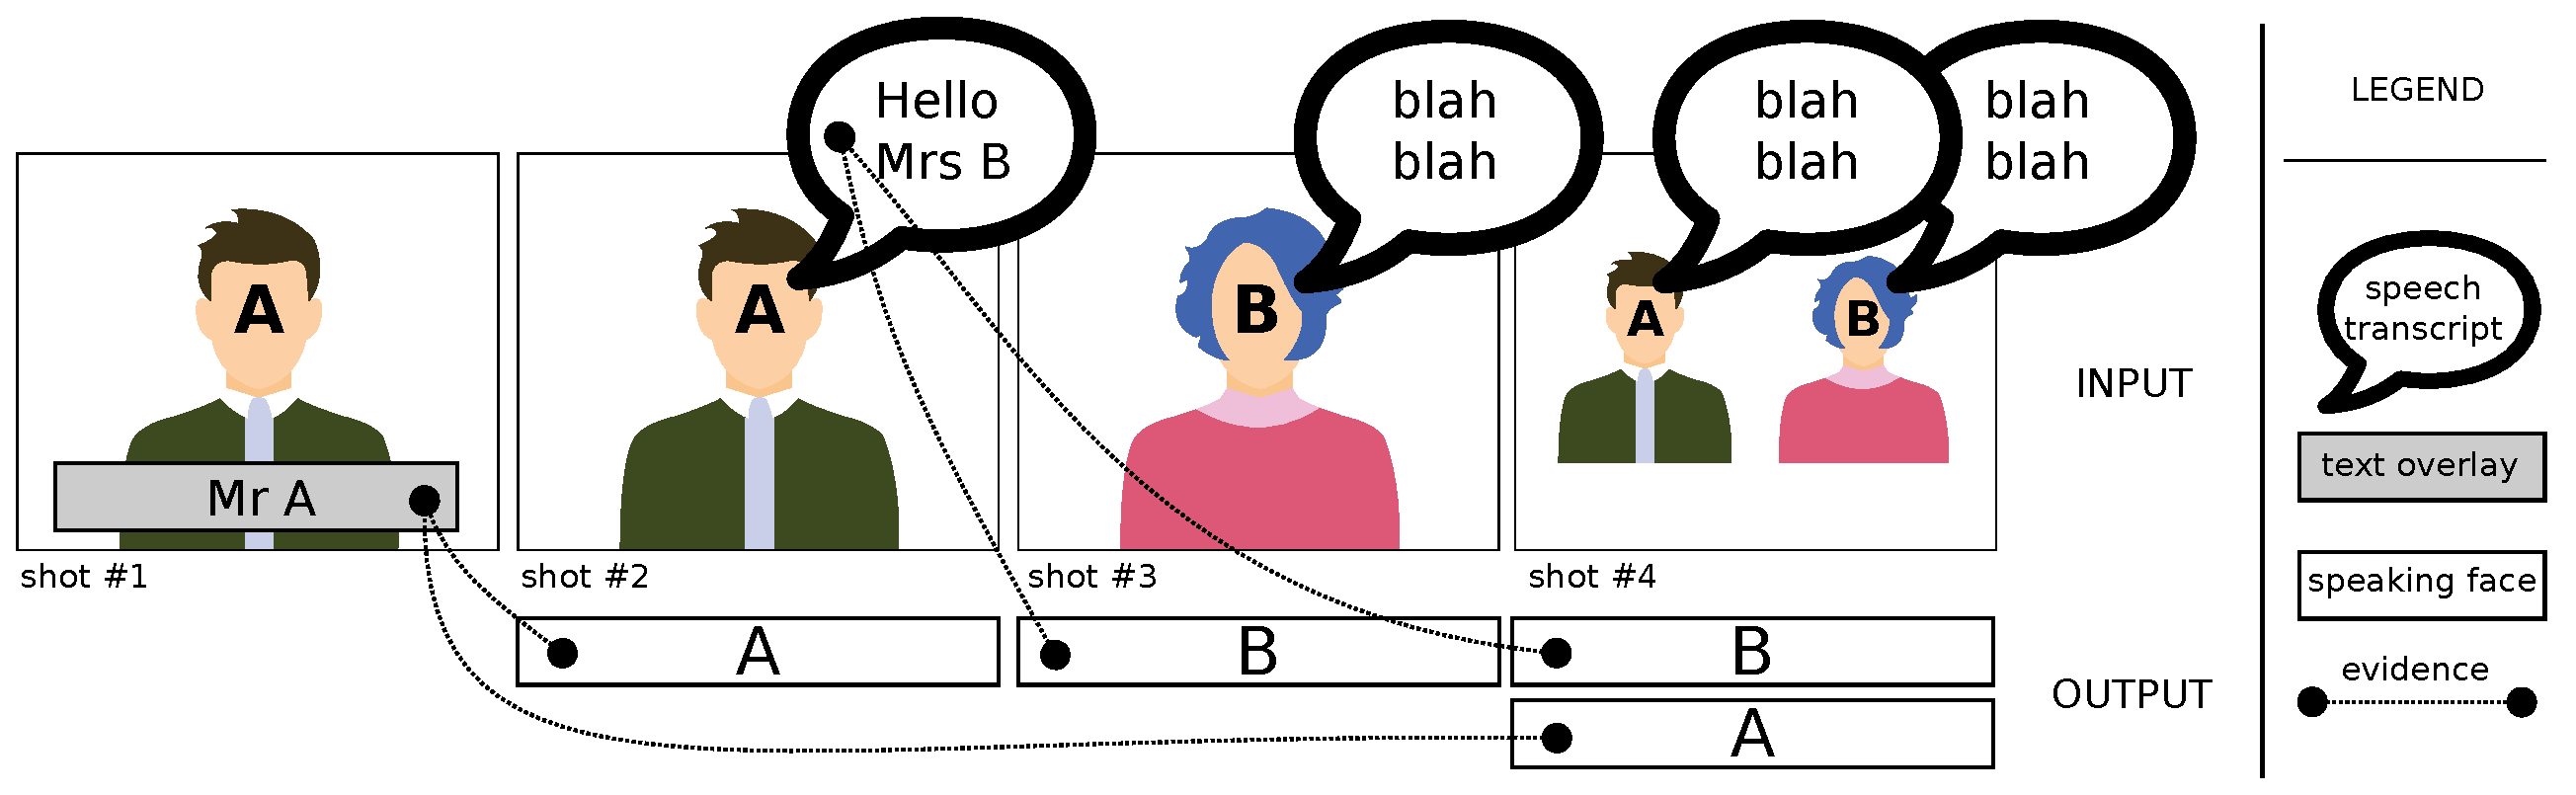
\includegraphics[width=1.\linewidth]{evidence.pdf}
\vspace*{-5mm}
 \caption{For each shot, participants have to return the names of every speaking face. An evidence is also returned for annotation process.}
\vspace*{-3mm}
 \label{fig:evidence}
\end{figure}

\mypartitle{Datasets and annotation.} The test set is divided into three sets: INA, DW and 3/24. The INA dataset contains a full week of broadcast for 2 TV channels for a total duration of 90 hours in French. The DW dataset~\cite{EUMSSI} is composed of video downloaded from Deutsche Welle website, in English and German for a total duration of 50 hours. The last dataset contains 13 hours of broadcast from 3/24 Catalan TV news channel. Each shot has been tagged with the names of people who appear and speak within that shot.

From all the submissions from participants, a set of hypotheses are generated for each shot. Then all participants also engaged in an interactive annotation process. During this process, detected names are first annotated with the corresponding thumbnails. Then a thumbnail is used to verify if the person appears in talks in a particular shot. The annotation process yields 3431 shots with 619 identities annotated. Further statistics on each set is presented in Tab. \ref{tab:stats}.

\begin{table}[tb]
\centering
\caption{Number of identities and corresponding shots where people appear and speak in each set of the corpus.}
\vspace*{-2mm}
\begin{tabular}{c|c|c|c|c|}
\cline{2-5}
    						   		& DW  	& INA 	& 3/24  & Total\\ \hline
 \multicolumn{1}{|c|}{\# shots} 		& 950	& 2250  & 231 & 3431\\ \hline

 \multicolumn{1}{|c|}{\# identities} 	& 344	& 232   & 44 & 619 \\ \hline
								
\end{tabular}
%
\vspace*{-5mm}
\label{tab:stats}
\end{table}



\mypartitle{Metrics.} The task is evaluated indirectly as an information retrieval task.%, using the following principle:
%
For each query $q \in \queries \subset \refNames$ (\texttt{first\-name\_lastname}), returned shots are first sorted by the edit distance between the hypothesized person name and the query $q$ and then by confidence scores.
Average precision $\text{AP}(q)$ is then computed based on the list of relevant shots (according to the groundtruth) and the sorted list of shots. Finally, Mean Average Precision is computed as follows:
\begin{align}
            \text{MAP} & = \frac{1}{|\queries|} \sum_{q \in \queries} \text{AP}(q) \nonumber
\end{align}

\mypartitle{Video OCR-NER}. As the task we aim at is full unsupervised, i.e. list of people is not provided in advance, their names have to be found in the audio (\emph{e.g.}, using ASR) or visual (\emph{e.g.}, using OCR) streams.
%
%Person identities can be retrieved either from speech transcripts or from overlaid person names commonly used to introduce the current speaker. 
%
Person identities from transcripts deteriorates when transcripts come from automatic speech recognition. Meanwhile, text can be reliably extracted using OCR techniques, and their association with people in the videos is easier than analysing whether or not pronounced names in ASR transcripts actually refer to people appearing in the video. Thus, in this work we use only names coming from OCR segments in videos.

To detect OCR segments in videos and exploit them for retrieval, we first relied on the approaches described in \cite{chen-pr04} for text recognition in videos, and on \cite{daddaoua:ICDAR:05} for text recognition and indexing.
%
In brief, given an input video, two main steps are applied: first the video is preprocessed with a motion filtering to reduce noise, and individual frames are processed to localize and binarize the text regions for text recognition.
%
%As compared to printed documents, OCR in TV news videos encounters several challenges: low resolution of text regions, sequence of different texts continuously displayed, or small amount of text to be recognized etc.
%
Multiple image segmentations of the same text region are decoded, and then all results are compared and aggregated over time to produce several hypotheses. 
%Due to the long running time, only the lower half of the videos are processed.
%
The best hypothesis is used to extract people names for identification. Then MITIE open library~\footnote{\url{https://github.com/mit-nlp/MITIE}} is used to recognize names from texts. 
%
%However, detecting names for identification can be more challenging due to several factors: (a) OCR text are often not sentences but short phrases, (b) names come from various languages, and (c) there are names of editorial staff who do not appear within the video, thus are not useful for identification such as cameramen or editors.
%
To improve the raw MITIE results, a heuristics step identifies names of editorial staff based on their roles (cameraman, editor, or writer) because they do not appear within the video, thus are not useful for identification.

\section{Overview of our approaches}
\label{sec:overview}

Conventional approaches for person recognition rely on the supervision of prior (face and/or voice) biometric models. Thus, a very large amount of trained models is needed to cover only a decent percentage of all the people in the show.
%
In addition, it is not always possible to predict which people will be the most important to find in the future.
%
To solve these problems, detected people names are assigned to faces and voices following the basic principal that occurrences with similar faces and voices should have the same name.
%

\mypartitle{Clustering-based naming (CBN).} This is the most common approach. Face/speech tracks are first aggregated into homogeneous clusters according to person identities. Then each clusters is tagged with the most probable person name (Fig.\ref{fig:cbn}). This approach heavily depends on the quality of clustering, especially over-clustering can significantly reduce the number of possible indices.

\mypartitle{Verification-based naming (VBN).} To overcome the weakness of CBN, verification-based naming puts higher priority on detected names. Face / speech tracks corresponding to names are used as enrolment data to train discriminative models. Names are then propagated to all face / speech tracks which are verified to have the same identity (Fig.\ref{fig:vbn}).

\mypartitle{Graph-based naming (GBN).} In verification-based naming, a name is propagated based on a one-one distance while in clustering-based naming, all the distances are globally considered. Graph-based naming is proposed as a hybrid approach to make use of both advantages.
A graph is built with a face/speech track as a node and weight of edges is the audio-visual similarity. Some nodes are initially tagged with the names similarly to verification-based naming. Names are then propagated along the edges within the graph (Fig.\ref{fig:gbn}).

As shown above, each of these approaches has different characteristics such as generic representation vs. discriminative models, pairwise verification vs. global optimization, etc..
%
To further investigate them, each of these approaches is described in full details in the following sections. 

\endinput